% !TeX root = ../main.tex

\chapter{Numerical model result}

\section{Reference model of Nazca}
\subsection{初始模型設定}
納茲卡模型,本研究建立一個長1200公里、深300公里的長方形二維剖面,包含一段長425公里的海洋岩石圈與775公里的大陸板塊,在兩個板塊交界處,建立一段長度26公里傾角50度的隱沒板塊,交接處區域的溫度較高,方便隱沒帶發育。
納茲卡板塊模型設計見圖\ref{fig::reference Nazca model}。

\begin{figure*}[hb]
    \centering
    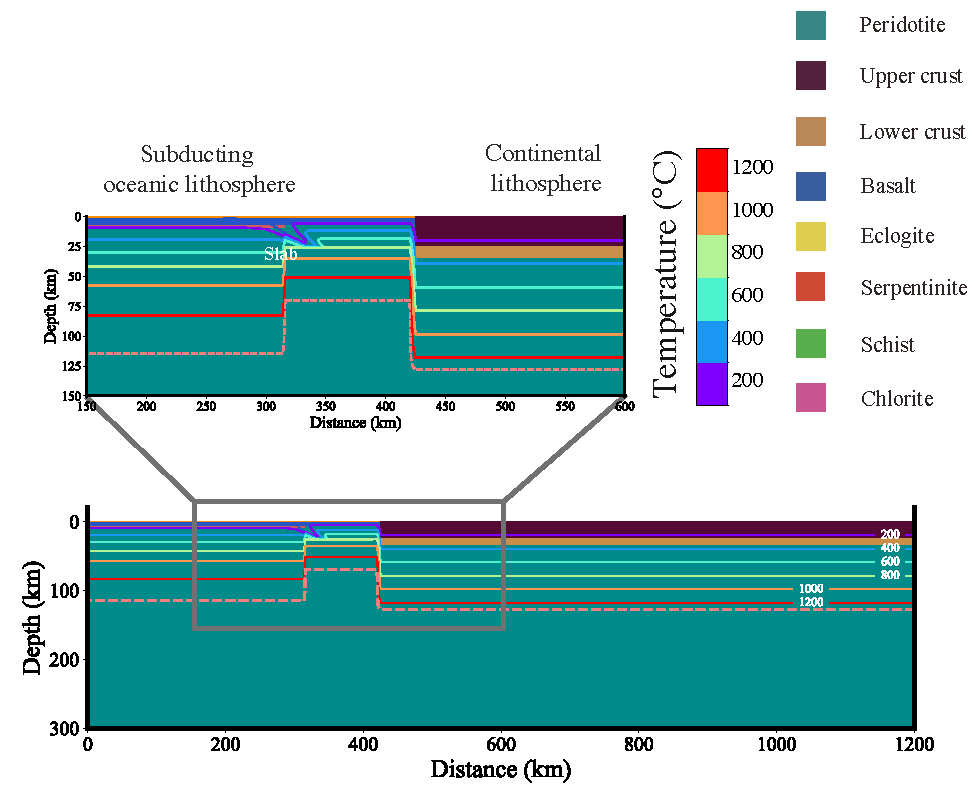
\includegraphics[width=6in]{Ref_Nazca.pdf}
    \caption[納茲卡板塊隱沒模型設計與邊界條件示意圖]{納茲卡板塊隱沒模型設計與邊界條件示意圖}
    \label{fig::reference Nazca model}
\end{figure*}


海洋岩石圈年齡為40個百萬年(\citealp{muller2019}),包含2公里厚的沈積物、6公里厚的玄武岩與10公里厚的含水橄欖岩,其熱構造由第二章式\ref{eq:Half Space Model}提及的半空間冷卻模型決定。
大陸岩石圈包含25公里厚的上部地殼(upper crust)與10公里厚的下部地殼(lower crust),由於秘魯與智利平坦隱沒區域的大陸地溫梯度資料較少,過去研究並沒有很好的約束,因此模型使用地溫梯度以每公里9.5度線性遞增至140公里深(\citealp{perez2008})至岩石圈底部1330度。
由於現生地震學觀測研究提及該地區地震活動度大,且地函岩石圈速度較高、板塊脫水作用不活躍,因此納茲卡模型的蛇紋岩厚度參數設定為5公里。模型左邊界以每年6公分速率往右移動,右邊界則固定不動。本研究參考的速度來自於\citealp{o2005uncertainties},使用印度-大西洋熱點參考座標(Indo-Atlantic hotspot reference frame)中的相對板塊運動模型計算(\citealp{schellart2008global})。

模型上邊界為自由表面,而下邊界則為開放邊界,物質可自由進出。
需要注意現今的秘魯與智利平坦隱沒區皆落在安地斯山脈造山範圍,然而本研究模型並沒有包含造山。
就現今觀測資料來看,平坦隱沒事件早於安地斯造山事件(\citealp{chen2019southward}; \citealp{hu2021southward}),兩者並沒有直接關係。


\subsection{模型結果}
納茲卡參考模型產生一深度約100-110公里、長度約300公里的平坦段。

在隱沒初始時期,隱沒作用促使地函流上湧,導致地函楔溫度升高,同時強烈的岩石變形與破壞導致隱沒板塊交界處產生摩擦熱,隱沒地殼溫度被動上升。
一系列的加溫導致岩石發生相變,隱沒地殼上的玄武岩相在約500度等溫線(深度40公里處)處相變成緻密的榴輝岩相,如圖\ref{fig::Nazca_Ref_26}a所示。
榴輝岩相密度遠大於周遭地函密度,造成隱沒系統中顯著的密度差不穩定,促使隱沒板塊驅動力產生,隱沒系統得以順利發育,隱沒帶密度剖面見圖\ref{fig::Nazca_Ref_26}c。

海洋地殼上的沉積物在隱沒過程中絕大比例留海溝處堆積,形成厚度約10公里的增積岩體,僅有約略10$\%$的沉積物被帶入地函中。
這些沉積物與海水被帶入地函內部,隨著地殼進入高溫高壓環境。
離開近地表後,地殼上的黏土礦物逐漸進入不穩定狀態,釋放出晶格中的水分,導致地函楔中的橄欖岩發生水合作用(hydration reaction)而相變成蛇紋岩化的橄欖岩(serpentinized peridotite),其與隱沒的沈積物一同在地函楔中形成強度低且密度較低的低黏滯度通道(low viscosity channel),見圖\ref{fig::Nazca_Ref_26}b與圖\ref{fig::Nazca_Ref_51}b黏滯度剖面。
在地函較深處,蛇紋岩化的橄欖岩進入更高溫的環境發生脫水,於深度70公里處相變回橄欖岩。

海洋板塊上的綠泥岩在120-130公里處發生脫水,相變成普通的橄欖岩。
綠泥岩脫水作用導致地函楔中的熔點下降,然而隱沒早期板塊溫度較低,即便進入地函楔中依然難以達到岩石熔點。

隱沒早期強烈的聚合作用在大陸岩石圈600度等溫線之上方產生一厚度25公里、寬度150公里的高壓帶,詳見圖\ref{fig::Nazca_Ref_26}d動態壓力剖面紅色區域。
該高壓帶在10 Myr變不復存在,隨著隱沒持續進行,低黏滯度通道導致地函楔頂部、板塊交界處壓力降低,於深度度80-120公里處形成低壓區,見圖\ref{fig::Nazca_Ref_51}d深藍色區域。 
低壓區域促使動水壓力力矩增加,導致隱沒板塊傾角(dip)快速降低(見圖\ref{fig::Nazca_Ref_slab_time})。

在模型進行10-15 Myr之間,低角度隱沒板塊下方因強烈彎曲(bending),在地函楔低壓區下方、隱沒地函岩石圈(subducting mantle lithosphere)處形成另一寬度約100公里的高壓區,見圖\ref{fig::Nazca_Ref_76}d紅色區域。
隱沒板塊上方的低壓帶與隱沒板塊下方的高壓帶所產生的壓力梯度恰好垂直於隱沒板塊,產生的動水壓力力矩快速增大,見圖\ref{fig::Nazca_Ref_torque_time},導致平坦隱沒於15 Myr後形成。

這段時間內因隱沒傾角漸緩,地函楔橄欖岩在壓力不變的情形下溫度逐漸上升,有部分岩石通過固相線,發生些許部分熔融事件,部分熔融位置於圖\ref{fig::Nazca_Ref_76}c中黃線處,部分熔融比例見圖\ref{fig::Nazca_Ref_melting_time}(a)。

隨後模型至30 Myr,平坦隱沒持續發育,大致維持800度等溫線深度,在模型中約略100-120公里深(圖\ref{fig::Nazca_Ref_76}a、\ref{fig::Nazca_Ref_101}a、\ref{fig::Nazca_Ref_126}a、\ref{fig::Nazca_Ref_150}a)。
隱沒板塊在900度等溫線前後離開平坦段,在深度120公里之後形成一高角度隱沒板塊。

因低黏滯度通道狹窄,隔絕地函流進入地函楔中,因此隱沒板塊上方的黏滯度持續維持低壓狀態。
此外,平坦隱沒上凹區域因強烈彎曲形成高壓帶,與低壓帶形成的壓力梯度同樣垂直於隱沒板塊,因此在20 Myr之後,與重力力矩相比,動水壓力力矩維持穩定優勢,隱沒板塊與上覆板塊被牢牢吸住(圖\ref{fig::Nazca_Ref_76}b, d、\ref{fig::Nazca_Ref_101}b, d、\ref{fig::Nazca_Ref_126}b, d、\ref{fig::Nazca_Ref_150}b, d)。


\begin{figure*}[htp]
    \centering
    \includegraphics[width=6in]{Ref_Nazcaframe_26_snapshot_5field_200.pdf}
    \caption[納茲卡參考模型於5 Myr時之結果。]{納茲卡參考模型於5 Myr時之結果。}
    \label{fig::Nazca_Ref_26}
\end{figure*}

\begin{figure*}[htp]
    \centering
    \includegraphics[width=6in]{Ref_Nazcaframe_51_snapshot_5field_200.pdf}
    \caption[納茲卡參考模型於10 Myr時之結果。]{納茲卡參考模型於10 Myr時之結果。}
    \label{fig::Nazca_Ref_51}
\end{figure*}

\begin{figure*}[htp]
    \centering
    \includegraphics[width=6in]{Ref_Nazcaframe_76_snapshot_5field_200.pdf}
    \caption[納茲卡參考模型於15 Myr時之結果。]{納茲卡參考模型於15 Myr時之結果。}
    \label{fig::Nazca_Ref_76}
\end{figure*}

\begin{figure*}[htp]
    \centering
    \includegraphics[width=6in]{Ref_Nazcaframe_101_snapshot_5field_200.pdf}
    \caption[納茲卡參考模型於20 Myr時之結果。]{納茲卡參考模型於20 Myr時之結果。}
    \label{fig::Nazca_Ref_101}
\end{figure*}

\begin{figure*}[htp]
    \centering
    \includegraphics[width=6in]{Ref_Nazcaframe_126_snapshot_5field_200.pdf}
    \caption[納茲卡參考模型於25 Myr時之結果。]{納茲卡參考模型於25 Myr時之結果。}
    \label{fig::Nazca_Ref_126}
\end{figure*}


\begin{figure*}[htp]
    \centering
    \includegraphics[width=6in]{Ref_Nazcaframe_150_snapshot_5field_200.pdf}
    \caption[納茲卡參考模型於30 Myr時之結果。]{納茲卡參考模型於30 Myr時之結果。}
    \label{fig::Nazca_Ref_150}
\end{figure*}

\subsubsection{參考模型脫水位置與岩漿作用}

\begin{figure*}[ht]
    \centering
    \includegraphics[width=6in]{Ref_Nazca_melting_time_v1.pdf}
    \caption[納茲卡參考模型岩漿作用隨時間變化]{納茲卡參考模型岩漿作用隨時間變化。}
    \label{fig::Nazca_Ref_melting_time}
\end{figure*}

\begin{figure*}[ht]
    \centering
    \includegraphics[width=6in]{Ref_Nazca_2Dtime_series.pdf}
    \caption[納茲卡參考模型部分熔融、岩漿庫與玄武岩相變時空關係圖]{納茲卡參考模型部分熔融、岩漿庫與玄武岩相變時空關係圖。}
    \label{fig::Nazca_Ref_2Dtime_series}
\end{figure*}

上述的剖面無法精確看到島弧位置,因為整個隱沒系統產生的島弧量非常少。
模型中發生部分熔融與海溝之距離隨時間變化如圖\ref{fig::Nazca_Ref_melting_time}a所示,。
普通的隱沒帶火山島弧與海溝的距離決大部分落在200公里以內,然而在納茲卡參考模型中,平坦隱沒的生成促使岩漿作用位置遠離海溝,並且隨著時間逐漸往內陸移動,最大可達近500公里。
除此之外,圖\ref{fig::Nazca_Ref_melting_time}a暗示著島弧往內陸移動速率變化,在25 Myr之前的島弧移動速率快速,斜率較大,然而在平坦隱沒發育後,島弧移動速率趨近緩和,斜率較小。

部分熔融量隨時間變化如圖\ref{fig::Nazca_Ref_melting_time}b。
在平坦隱沒發育穩定後,隱沒板塊進入大陸岩石圈內側,不斷將地函楔溫度降低。
因此在平坦隱沒形成後5個百萬年之內,岩石熔融量快速減少,至30 Myr後每20萬年僅有不到1立方公里岩石熔融。
圖中顯示岩漿作用活躍度在20 Myr前後達到高峰,並且在平坦隱沒發育後有些微沉積物熔融的現象,此現象與該地區的岩漿觀測資料吻合。

將模型中部分熔融事件與岩漿庫絕對位置繪出,分別獲得圖\ref{fig::Nazca_Ref_2Dtime_series}b, c。在模型中10-25 Myr時,部分熔融與岩漿庫快速往內陸移動,隨後在30-50 Myr後部分熔融事件與岩漿庫位置維持穩定,表示模型已達動態平衡。

玄武岩至榴輝岩相變位置見圖\ref{fig::Nazca_Ref_2Dtime_series}c。
玄武岩相變位置在早期約50公里深,而直到30 Myr已經來到80公里深,並且有逐漸遠離海溝的趨勢。
由於隱沒系統持續穩定隱沒,導致近海溝側溫度逐漸變冷,因此玄武岩相變也往更深且更內陸的方向移動,最終在約80公里深,橫軸座標450-460公里左右收斂。
儘管該結果顯示玄武岩相變有逐漸延遲的現象,然而其相變深度仍然早於平坦隱沒深度,因此,可確認玄武岩相變延遲並不足以解釋平坦隱沒由尚未相變得海洋地殼所構成。

\subsubsection{參考模型隱沒板塊與其轉動平衡}

模型中的平坦隱沒長度與深度隨時間變化見圖\ref{fig::Nazca_Ref_slab_time}a, b,平坦段深度與長度的定義已於\ref{平坦隱沒定義}提及,平坦段被定義為隱沒板塊上兩個反曲點之間的區域,平坦段長度為隱沒板塊上兩個反曲點之間的長度,而平坦深度為平坦段中的深度中位數。
在平坦隱沒發育初期,模型進行20-30 Myr之間,因動水壓力力矩持續增加,且大陸岩石圈溫度不斷降低,岩石800度等溫線不斷往內陸移動,因此平坦隱沒段隨時間推進逐漸變長,至30 Myr達到200公里左右。儘管平坦隱沒段長度逐漸變長,然而模型中平坦隱沒段深度並沒有劇烈改變,皆落在110-120公里深。
在大約30 Myr 後平坦隱沒長度並沒有太大變化,平坦深度約在10公里內移動,可以視為系統已達到動態平衡。

模型中隱沒板塊於150公里之內的角度變化如圖\ref{fig::Nazca_Ref_slab_time}c。
在模型早期,角度隨時間陡降,然而在20 Myr後便沒有太大起伏,達到穩定最小值。
直得注意的是,動水壓力力矩幾乎在同時間達到穩定大值,如圖\ref{fig::Nazca_Ref_slab_time}所示,於20 Myr後不再有顯著下降或上升。

\begin{figure*}[hb]
    \centering
    \includegraphics[width=5in]{Ref_Nazca_slab_time_v1.pdf}
    \caption[納茲卡參考模型隱沒板塊狀態隨時間變化]{納茲卡參考模型隱沒板塊狀態隨時間變化。}
    \label{fig::Nazca_Ref_slab_time}
\end{figure*}


隱沒帶中重力力矩解析解由下式定義:

\begin{align}
    t_G=\int^l_0 \Delta\rho(r,\alpha)ghr\ cos\alpha\ dr
    \label{eqn:Gravity Torque}
\end{align}
改寫自\citealp{stevenson1977angle},其中$l$為隱沒板塊長度,$\Delta\rho$為隱沒板塊與周遭地函密度差,$\alpha$為隱沒板塊與水平的夾角,$r$為與轉動支點的徑向座標,$g$為重力加速度,$h$為隱沒板塊厚度。

由於\ref{eqn:Gravity Torque}假設隱沒帶為一類似\ref{fig::Torque_ana}的模型,隱沒系統已達轉動平衡且隱沒板塊在二維剖面上是一線性構造,因此$\alpha$不變且為一常數。

\begin{figure*}[hb]
    \centering
    \includegraphics[width=3in]{Torque_ana.png}
    \caption[簡易隱沒帶二為剖面示意圖]{簡易隱沒帶二為剖面示意圖。}
    \label{fig::Torque_ana}
\end{figure*}

動水壓力力矩解析解由下式定義:
\begin{align}
    t_H=\int^l_0 [P_{sub}(r)-P_{wedge}(r)]r\ dr
    \label{eqn:Hydrodynamic Torque}
\end{align}
改寫自\citealp{McKenzie1969},其中$P_{sub}$為隱沒板塊下的壓力,$P_{wedge}$為隱沒板塊上、地函楔的壓力,壓力的解析解計算方式如下:

\begin{align}
    P_{sub}=\frac{2 \eta U sin \alpha}{r[(\pi - \alpha)+sin\alpha]}
    \label{eqn:Psub}
\end{align}

\begin{align}
    P_{wedge}=-\frac{2 \eta U sin^{2} \alpha}{r(\alpha^2-sin^2\alpha)}
    \label{eqn:Pwedge}
\end{align}

$U$為隱沒板塊隱沒速度,$\eta$為地函黏滯度,在穩態解析解中皆視為常數。$t_G$與$t_H$單位與力矩相當,皆為$N\cdot m$。

過去的平坦隱沒數值模型研究利用解析解的方式計算模型中的重力力矩與動水壓力力矩,然而上式\ref{eqn:Gravity Torque}至\ref{eqn:Pwedge}中假設隱沒系統已達平衡,許多參數皆為常數,並且模型假設隱沒板塊為一線性構造,有過於簡化的疑慮。
因此本研究利用數值解的結果計算模型中不同時間點,在假設海溝為支點的情況下,獲得隱沒板塊所受的重力力矩與動水壓力力矩。

\begin{align}
    \tau_{gravity} =  g\sum ^L_{l=0} \Delta \rho(l)\ r(l)\ cos\ \alpha (l)\ V(l) 
    \label{eqn:}
\end{align}

\begin{align}
    \tau_{suction} =  \sum ^L_{l=0} [P_{sub}(l)-P_{wedge}(l)]\cdot dl\cdot r(l)\ cos\ \alpha (l)
    \label{eqn:}
\end{align}

計算每段隱沒板塊截面上的密度差與總體積,對整段隱沒板塊積分,
獲得隱沒板塊所受的重力力矩與動水壓力力矩



\begin{figure*}[hb]
    \centering
    \includegraphics[width=6in]{Ref_Nazca_torque_time.pdf}
    \caption[納茲卡參考模型重力力矩與動水壓力力矩隨時間變化]{納茲卡參考模型重力力矩與動水壓力力矩隨時間變化。}
    \label{fig::Nazca_Ref_torque_time}
\end{figure*}

至於模型產生大量東水壓力矩的原因,
我們初步判斷可能由mantle wedge中的年制度所決定。
若將模型的蛇紋岩厚度增加至6公里
.....




除蛇紋岩之外,額外測試岩漿參數,獲得不同的低年制度厚度於mantle wedge中的發育情形。

